% This is samplepaper.tex, a sample chapter demonstrating the
% LLNCS macro package for Springer Computer Science proceedings;
% Version 2.25 of 2026/09/03
%
\documentclass[runningheads]{llncs}
%
\usepackage[T1]{fontenc}
% T1 fonts will be used to generate the final print and online PDFs,
% so please use T1 fonts in your manuscript whenever possible.
% Other font encondings may result in incorrect characters.
%

\usepackage{newtxtext}       % 
\usepackage[varvw]{newtxmath}       % selects Times Roman as basic font

%\hypersetup{hidelinks}
\usepackage[hidelinks]{hyperref}
\usepackage{graphicx}
\usepackage{placeins}
\usepackage{array}
\usepackage{xurl}
\setlength{\emergencystretch}{2em}
% Used for displaying a sample figure. If possible, figure files should
% be included in EPS format.
%
% If you use the hyperref package, please uncomment the following two lines
% to display URLs in blue roman font according to Springer's eBook style:
%\usepackage{color}
%\renewcommand\UrlFont{\color{blue}\rmfamily}
%\urlstyle{rm}
%
\begin{document}
%
\title{Producer Activity and Relative Exposure in an Adaptive Social Network}
%
\titlerunning{Producer Activity and Relative Exposure}
% If the paper title is too long for the running head, you can set
% an abbreviated paper title here
%
\author{Kajetan Karbowski (s5470161) \and
Karolina Kozikowska (s5504503)}
%
% First names are abbreviated in the running head.
% If there are more than two authors, 'et al.' is used.
%
\institute{Design of Multi-Agent Systems, University of Groningen}
%
\maketitle              % typeset the header of the contribution
%
\begin{abstract}
High-volume AI-generated content motivates a basic question: how does producer activity affect exposure relative to production? We study this question using DOCES, an adaptive social-network model extended with weighted activation, persistent post provenance, and feed-receipt tracking. The synthetic label identifies a producer subgroup; it does not encode content quality or an adaptive production strategy. Across 10,000 independent worlds, we vary subgroup prevalence from 1\% to 25\% and relative activity from 1\(\times\) to 15\(\times\). With a one-item feed, mean relative exposure \(D=S_{\mathrm{exposure}}-S_{\mathrm{production}}\) is slightly positive at moderate activity and negative at high activity. Descriptive interpolated zero crossings lie between 4.67\(\times\) and 5.28\(\times\). A separate experiment with 200 paired worlds tests feed capacities 1, 5, and 20. High-activity mean relative exposure remains negative in the tested conditions, but the moderate-activity pattern and effect magnitude depend on capacity. The study isolates activity and prevalence as two components relevant to AI-slop distribution. It does not model the production--reward feedback process or establish how real AI-generated content is ranked or consumed.
\keywords{Multi-agent systems \and Synthetic content \and Information diffusion \and Social media \and Agent-based modelling \and AI slop}
\end{abstract}

\section{Introduction}

Generative AI enables online content producers to produce content at a scale that would previously have required substantially more manual effort~\cite{tang2026}. This has contributed to the growth of high-volume AI-generated material that is often described as AI slop. We use the term \emph{AI slop} for the motivating real-world phenomenon, while the model represents content more generally as human- or synthetic-origin content. Recent ethnographic work by Tang et al.~\cite{tang2026} shows that some producers systematically benchmark viral content, test variations, operate multiple accounts, and prioritise speed, scale, and adaptability over stable authorship or identity.

A high production volume alone does not tell us how much synthetic content users actually receive. Social-media content spreads through interactions between producers, users, social connections, reposting behaviour, and recommendation systems. A minority of highly active producers may therefore obtain either more or less exposure than their raw production share would suggest.

The distinction matters because a large share of synthetic content in users' feeds can arise for different reasons. Synthetic producers may simply create more posts, or network and platform dynamics may give those posts more exposure than their production share would predict. These mechanisms have different implications for understanding high-volume AI-generated content. Empirical work on AI-slop production documents strategies centred on scale, rapid iteration, and attention capture~\cite{tang2026}, while Pendergrass et al.~\cite{pendergrass2025} frame user attention as a scarce resource for which such content competes. We therefore study not only how much synthetic content is produced, but how efficiently that production translates into exposure.

We study the following research question:

\begin{quote}
\textit{How do producer activity and prevalence affect a labelled subgroup's share of feed receipts relative to its share of production in DOCES?}
\end{quote}

We define relative exposure as
\[
D = S_{\mathrm{exposure}} - S_{\mathrm{production}},
\]
where positive values indicate that synthetic-origin content receives a larger
share of feed exposure than its share of production, while negative values
indicate attenuation.

We address the main question through three subquestions:
\begin{enumerate}
    \item \textit{SQ1}. How does synthetic-agent activity affect
    synthetic-content production share and exposure share?
    \item \textit{SQ2}. How does synthetic-producer prevalence modify the
    effect of activity on relative exposure?
    \item \textit{SQ3}. Is the relationship between synthetic activity and
    relative exposure monotonic, or does it reverse at high activity levels?
\end{enumerate}

In the present experiment, ``synthetic'' denotes the provenance of posts introduced by a randomly assigned producer subgroup. These agents follow the same posting, reposting, opinion, and network rules as other agents. Only their activation weight differs. The label could equally identify another high-activity producer group; the simulator does not generate or classify AI content.

Our contribution is a controlled study of two components relevant to AI-slop distribution: producer prevalence and activity. We do not test whether AI generation itself causes amplification or whether producers learn successful strategies. We add a focused feed-capacity sensitivity experiment to assess whether the main result depends on the one-item feed.

These questions are measurable through production, feed-receipt, and activity statistics recorded by the simulation. We vary both synthetic-producer prevalence and relative activity while measuring the resulting production and exposure shares.

A multi-agent model is appropriate because relative exposure is not determined by producer activity alone. It emerges from repeated interactions between heterogeneous users, posting and reposting, limited feeds, content filtering, opinion dynamics, and adaptive network connections. The simulation allows us to vary producer activity while holding the remaining model mechanisms fixed.

\section{Related Work}

\subsection{Information diffusion and opinion dynamics}
Our main computational starting point is the model by Oliveira et al.~\cite{oliveira2026}. Their agent-based model combines information diffusion with opinion dynamics on an adaptive social network. Agents have limited feeds, create or repost content, receive content according to filtering rules, update their opinions, and may rewire social connections. The authors show that reposting, recommendation rules, and the probability of introducing new content can substantially change both cascade dynamics and final opinion distributions.

This model is particularly useful for our research because it explicitly links individual posting behaviour to network-level information diffusion. It also provides an existing mechanism for recommendation, reposting, limited attention, and adaptive network structure.

We use the DOCES implementation developed by de Arruda et al.~\cite{deArruda2025}. DOCES provides the adaptive social-network simulation and supports recommendation rules, changes in friendships, and opinion dynamics.

\subsection{Critical review of Oliveira et al.}
Oliveira et al. provide a strong starting point because their model separates several mechanisms that are often combined in empirical social-media data. The authors can independently manipulate content innovation, recommendation, rewiring, and opinion updating. They also compare simulated cascade distributions with empirical data, which gives the model more grounding than a purely abstract diffusion model.

The model nevertheless makes one simplifying assumption that is central to our research question: users are selected uniformly for activation. All users therefore have the same opportunity to create or repost content. Oliveira et al.~\cite{oliveira2026} explicitly identify heterogeneous activity and bursty dynamics as directions for future work.

This assumption is poorly suited to the production practices described by Tang et al.~\cite{tang2026}, where some AI-supported producers operate at high volume. We therefore retain the Oliveira diffusion dynamics but replace uniform activation with heterogeneous activity weights.

\subsection{Synthetic content and the attention economy}

Tang et al.~\cite{tang2026} provide behavioural grounding for our synthetic producers. Their ethnographic study of AI-slop creators in China describes production practices based on high output, repeated experimentation, benchmarking successful formats, matrix account systems, and algorithmic opportunism. Their findings suggest that AI-supported production can make speed and scale central features of online content production.

Pendergrass et al.~\cite{pendergrass2025} describe a related conceptual feedback process. They argue that cheap AI production, attention-oriented content, platform distribution, and economic incentives can form a self-reinforcing cycle. Their framework emphasizes that generated content competes for attention and that successful attention strategies create incentives for further production.

These studies serve different roles. Tang et al. provide qualitative motivation for heterogeneous activity; they do not supply numerical values for our activity multipliers. Pendergrass et al. provide a conceptual account of creation, distribution, and reward, rather than an empirically calibrated diffusion rule. We model a fixed activity advantage, not this feedback cycle. In particular, adaptive network rewiring in DOCES is not adaptive producer strategy.

\subsection{Research gap}

The three strands of work provide complementary pieces of the problem. Oliveira et al.~\cite{oliveira2026} provide a mechanistic model of posting, reposting, recommendation, limited attention, opinion change, and adaptive network structure, but assume uniform user activation. Tang et al.~\cite{tang2026} document synthetic-content production practices centred on high output and rapid experimentation, while Pendergrass et al.~\cite{pendergrass2025} emphasise competition for limited attention.

What remains unclear is how a systematically high-activity producer population affects exposure once its content enters an adaptive social network. In particular, higher production need not imply proportionally higher exposure. Our contribution is therefore to introduce heterogeneous activity into the Oliveira--DOCES framework and explicitly separate synthetic production share from synthetic exposure share.

\section{Method}

\subsection{Base model}

We build on the adaptive social-network model of Oliveira et al.~\cite{oliveira2026}, using its DOCES implementation by de Arruda et al.~\cite{deArruda2025}. Each user \(i\) is a node in a directed network and holds a continuous opinion \(b_i\in[-1,1]\). Each piece of content has a fixed opinion value \(\theta\in[-1,1]\), and each user maintains an ordered feed (memory) of size \(\alpha\).

One simulation iteration consists of five stages. First, one user \(i\) becomes active. In the original model this user is selected uniformly; our heterogeneous-activity extension modifies only this stage. Second, with probability \(\mu\), the active user creates new content whose opinion \(\theta\) is sampled uniformly from \([-1,1]\). With probability \(1-\mu\), the active user instead selects the highest-priority item in its feed for reposting, provided the feed is non-empty. The selected item's feed priority is subsequently rotated to the lowest priority. In the main sweep, \(\alpha=1\), so this reordering has no effect on which item remains in the feed. It matters in the larger-feed sensitivity conditions.

Posting is accepted probabilistically according to the conflicting-posting filter used by Oliveira et al.:
\[
P_p(\theta,b_i)=
\cos^2\left(\frac{\pi}{2}|\theta-b_i|\right).
\]
If the post is made, each follower \(j\) independently receives it according to
\[
P_r(b_i,b_j,\phi)=
\cos^2\left(\frac{\pi}{2}|b_i-b_j|+\phi\right),
\]
where \(\phi\) controls the receiving rule and acts as a stylised proxy for platform recommendation. The filter acts only on existing follower links. It does not rank candidate content or recommend posts outside this network. At \(\phi=\pi/2\), it favours opinion distances near 1 and suppresses distances near 0 and 2; it is not a general measure of recommendation strength. A post that passes the filter enters the top of a follower's feed only if it is absent there. When the feed is full, insertion removes the lowest-priority item. DOCES can still update a recipient's opinion after filter acceptance when the post is already present; such an interaction adds no receipt to our exposure measure.

Recipients update their opinions through either attraction to or repulsion from the received post. With the opinion range fixed to \([-1,1]\), the probability of attraction for recipient \(j\) is
\[
P_{\mathrm{attr}}(\theta,b_j)
    = 1-\frac{|\theta-b_j|}{2},
\]
and repulsion occurs otherwise. Under attraction, \(b_j\) moves by at most \(\Delta\) towards \(\theta\), without overshooting the post opinion. Under repulsion, \(b_j\) moves by \(\Delta\) away from \(\theta\) and is clipped to the interval \([-1,1]\). No stubborn agents are used in the reported experiments.

When rewiring is enabled, DOCES considers rewiring only after a repulsive interaction. Let \(b'_j\) denote the recipient's opinion after repulsion and let \(y=|b_i-b'_j|\) be its distance from the active user's opinion. Rewiring is possible only when \(y>1\). In the implementation used here it occurs when
\[
u > \cos^2\left(\frac{\pi}{2}y\right),
\qquad u\sim U(0,1).
\]
Equivalently, conditional on \(y>1\), the implemented rewiring probability is \(1-\cos^2(\pi y/2)\). When rewiring succeeds, the existing follower connection to the active user is replaced by a connection to a randomly sampled eligible user; the current source, the recipient itself, and already-connected targets are excluded. Thus information diffusion, opinion dynamics, and network structure can co-evolve during a simulation.

\subsection{Baseline parameterisation}

Unless otherwise stated, all reported experiments use
\[
N=1000,\qquad
\mu=0.1,\qquad
\phi=\frac{\pi}{2},\qquad
\Delta=0.1,\qquad
\alpha=1,
\]
with rewiring enabled and 100,000 requested iterations per simulation. The inherited inclusive loop executes 100,001 activations for this request. We retain this convention in both experiments. Initial
opinions are sampled independently and uniformly from \([-1,1]\). Agents are
connected by a directed Erdős--Rényi graph. For each ordered pair of distinct
agents, an edge is sampled independently with probability
\[
p=\frac{10.21}{N-1},
\]
giving a target mean in-degree of 10.21.

These choices are inherited from the Oliveira et al. parameterisation used in our baseline validation rather than fitted to synthetic-content data. In particular, Oliveira et al. use an Erdős--Rényi network with \(N=1000\), \(\phi=\pi/2\), \(\Delta=0.1\), and feed size \(\alpha=1\) when characterising the effect of innovation and reposting~\cite{oliveira2026}. We retained this configuration so that heterogeneous activity could be introduced while keeping the remaining diffusion dynamics close to a previously characterised setting.

The Erdős--Rényi network and one-item feed should therefore be interpreted as controlled modelling assumptions, not as literal representations of a specific social-media platform. In particular, \(\alpha=1\) creates a strong limited-attention regime. Section~\ref{sec:feed-design} tests larger feeds. Alternative network structures remain untested.

\subsection{Assumptions and their relevance to AI slop}

We retain the base model to isolate activity, but inherited choices also constrain interpretation (Table~\ref{tab:assumptions}). None of these parameters is fitted to AI-slop traffic.

\begin{table}[tb]
\caption{Model choices, their purpose, and their interpretive limits.}
\label{tab:assumptions}
\centering\small
\begin{tabular}{>{\raggedright\arraybackslash}p{0.22\linewidth}>{\raggedright\arraybackslash}p{0.32\linewidth}>{\raggedright\arraybackslash}p{0.36\linewidth}}
\hline
Choice & Purpose & Limit for AI-slop interpretation \\\hline
Fixed activity weights and random producer labels & Isolate output opportunities and subgroup prevalence & No learning, burstiness, coordinated accounts, or preferential producer placement \\[4pt]
Common innovation probability and uniform new-post opinions & Hold content-generation rules fixed & No difference in quality, format, topic targeting, or generation cost \\[4pt]
Directed random graph & Allow follower diffusion with controlled initial degree & No calibrated hubs, communities, or real platform network \\[4pt]
Opinion filters and rewiring & Retain feedback between diffusion and user connections & No learned recommender, engagement reward, or producer response to success \\[4pt]
Finite ordered feeds & Limit retained repost opportunities & Memory is not measured viewing time; capacity also affects repeat-receipt suppression \\\hline
\end{tabular}
\end{table}

Increasing an activation weight increases opportunities to repost as well as to create new posts. It therefore approximates high account activity rather than a pure increase in original-content production. Moreover, the total activation budget is fixed. Increasing synthetic activity lowers the expected number of human activations within that budget. We study a change in relative activity allocation, not additional posts over a calibrated amount of real time.

\subsection{Baseline validation}

Before introducing heterogeneous activity, we validated the simulator against the qualitative behaviour reported in Fig.~2 of Oliveira et al.~\cite{oliveira2026}. Using the corresponding baseline configuration, we ran 50 simulation seeds while holding the network and initial opinions fixed. The low-innovation condition \(\mu=0.1\) produced larger cascades and more frequent bimodal opinion distributions: 15 of 50 runs exceeded the bimodality criterion, compared with 1 of 50 at \(\mu=1\). The median maximum cascade sizes were 2232.5 and 1, respectively. This reproduces a qualitative contrast, not universal polarisation at low innovation. We repeated this baseline after implementing our simulator extensions and obtained the same representative results when activity weighting was disabled. We therefore used this as a regression validation rather than claiming an exact numerical replication.

\subsection{Heterogeneous activity}
We extended DOCES with a relative activity weight \(w_i\) for each user \(i\). The probability of selecting agent \(i\) is

\[
P(i)=\frac{w_i}{\sum_j w_j}. 
\]

Human agents receive weight 1. Synthetic agents receive an activity multiplier \(m\). No other behavioural rule depends on the synthetic label. Synthetic and human agents use the same content-creation probability, posting and receiving filters, opinion dynamics, and rewiring rule. The experimental intervention therefore isolates differences in activation frequency.

For \(N_s\) synthetic and \(N_h\) human agents, the expected synthetic activation share is therefore

\[
S_{\mathrm{activation}} = \frac{N_s m}{N_h + N_s m}. 
\]

We validated the implementation independently. A two-agent test with weights 9 and 1 resulted in observed activation shares of approximately 0.900 and 0.100 over 100,001 selections.

When activity weights are not configured, DOCES follows its original uniform selection procedure. We reran the Oliveira baseline after the extension and obtained the same representative simulation results.

\subsection{Post provenance and exposure}
Each newly created post stores the identifier of its original creator. Reposts retain both the post identifier and original creator, so exposure is attributed to the producer that originally introduced the content rather than to the user currently reposting it.

DOCES initializes each feed with \(\alpha\) distinct background posts. We assign these posts an origin ID of \(-1\) and exclude them and their receipts from the human-versus-synthetic measurements. They still occupy feeds and can be reposted, so they influence subsequent dynamics. Larger capacities therefore also increase the initial background stock from \(N\) to \(N\alpha\) posts.

We define one model-level exposure event as a successful insertion of a post into another user's feed. The receiving filter must accept the post, and the same post must not already be in the recipient's feed. We do not count insertion into the posting user's own feed as exposure.

This measure represents successful feed receipt inside the model. It should not be interpreted as an exact real-world impression or view.

\subsection{Outcome measures}
We measure synthetic production share as

\[
S_{\mathrm{production}} = \frac{N_{\mathrm{synthetic\ posts}}} {N_{\mathrm{synthetic\ posts}}+N_{\mathrm{human\ posts}}}.
\]

Synthetic exposure share is

\[
S_{\mathrm{exposure}} = \frac{R_{\mathrm{synthetic}}} {R_{\mathrm{synthetic}}+R_{\mathrm{human}}},
\]

where \(R\) is the number of successful feed receipts. Production counts distinct new posts accepted by the posting filter, not rejected creation attempts or reposts. A post can contribute several receipts to the same recipient if it leaves that feed and is later reinserted. Receipts therefore measure neither unique audience reach nor time spent viewing content.

Our primary outcome is

\[
D = S_{\mathrm{exposure}}-S_{\mathrm{production}}.
\]

A positive value indicates that synthetic content obtains more exposure than its production share. A negative value indicates attenuation.

To examine how efficiently additional production translates into exposure, we also calculate mean receipts per post separately for synthetic and human content:
\[
E_s = \frac{R_{\mathrm{synthetic}}}{N_{\mathrm{synthetic\ posts}}},
\qquad
E_h = \frac{R_{\mathrm{human}}}{N_{\mathrm{human\ posts}}}.
\]

We use
\[
G_E = E_s-E_h
\]
as an exposure-efficiency gap. A positive value means that the average synthetic-origin post receives more successful feed receipts than the average human-origin post; a negative value means it receives fewer. These measures are algebraically related. If \(q=S_{\mathrm{production}}\), then, whenever the denominators are positive,
\[
D=\frac{q(1-q)(E_s-E_h)}{qE_s+(1-q)E_h}.
\]
Thus the signs of \(D\) and \(G_E\) agree by construction; they are not independent evidence for a causal mechanism.

\subsection{Experimental design}

We test synthetic-producer prevalence values of
\[
1\%,\;5\%,\;10\%,\;15\%,\;20\%,\;25\%
\]
and relative activity multipliers of
\[
1,\;2,\;3,\;5,\;7.5,\;10,\;15.
\]
A 0\% synthetic control is evaluated at baseline activity. The factorial design therefore contains \(6\times7=42\) positive-prevalence conditions plus one control, giving 43 conditions in total. The 0\% control is used as an implementation reference and is excluded from factorial prevalence--activity inference because an activity multiplier is not defined for a population containing no synthetic agents.

The four seeds for each world are generated deterministically from master seed \texttt{20260924}. The complete seed manifest is stored with the experiment outputs.

For each world, the master generator produces four separate seeds: a network seed, initial-opinion seed, producer-assignment seed, and simulation seed. All experimental conditions within that world reuse these four seeds. They therefore share the same initial network, initial opinions, producer ordering, and simulation seed. All four seeds change between worlds, creating paired comparisons within worlds while keeping different worlds independent.

We generated 10,000 independent simulated worlds for the final sweep to obtain stable estimates of the condition means and uncertainty intervals. Smaller 2,000- and 5,000-world checkpoints produced the same qualitative relationship; the larger run mainly reduced Monte Carlo uncertainty.

Synthetic groups are nested within each world. A random producer ordering is generated once per world, and larger synthetic populations extend smaller ones. For example, the 5\% synthetic group contains the same agents as the 1\% group plus additional agents. This reduces unnecessary variation in producer identity between prevalence conditions.

The complete design contains
\[
10{,}000 \times 43 = 430{,}000
\]
unique condition-runs.

\subsection{Focused feed-capacity experiment}
\label{sec:feed-design}

We run a separate sensitivity experiment with 200 independent worlds generated from master seed \texttt{20261022}. We cross feed capacities \(\alpha\in\{1,5,20\}\), producer prevalences \(\{5\%,25\%\}\), and activity multipliers \(\{1,3,15\}\). This gives 18 conditions per world and 3,600 condition-runs. We retain the main sweep's network size, degree, filters, innovation probability, opinion update, rewiring, and requested iteration count. Each world shares its graph, initial opinions, nested producer assignment, and simulation seed across conditions.

We selected 3\(\times\) and 15\(\times\) to contrast moderate and high activity after observing the main sweep. The experiment is therefore an exploratory sensitivity analysis. It is not a second 10,000-world sweep or a new search for a turnover threshold. We report pointwise 95\% Student's \(t\) intervals for condition means and for paired within-world differences \(D_{15}-D_3\), without multiplicity adjustment. The same seed does not keep random draws aligned after conditions diverge; different feed sizes also require different numbers of initialization draws.

Changing capacity modifies retention, repost order, duplicate suppression, and the initial stock of background posts together. This experiment tests the bundled feed-capacity assumption. It does not separate feed displacement from other capacity-dependent effects.

\subsection{Statistical analysis}

For each main-sweep condition, we report the mean and a 95\% Student's \(t\) confidence interval for the mean across 10,000 independent worlds. Since activity conditions within each world share the same network, initial opinions, producer ordering, and simulation seed, activity comparisons use paired within-world differences.

For omnibus inference, we represent the \(D\) values from all prevalence-activity conditions as a repeated-measures vector for each world. We test contrasts of the across-world mean vector using its empirical covariance matrix, producing Wald \(\chi^2\) tests for prevalence, activity, and their interaction.

We additionally evaluate exploratory paired activity contrasts using two-sided paired \(t\)-tests. We consider three contrast families: comparisons of each activity level against \(1\times\), comparisons against \(3\times\), and comparisons between adjacent activity levels. Holm's method is applied separately within each family across all tested prevalence levels. For these contrasts we report the mean paired difference, its 95\% confidence interval, and paired Cohen's \(d_z\). Given the large number of independent worlds, interpretation emphasises estimated effect sizes and uncertainty rather than statistical significance alone.

For a paired difference \(\Delta D\), paired Cohen's effect size is
\[
d_z=\frac{\overline{\Delta D}}{s_{\Delta D}}.
\]

For descriptive analysis of the turnover, we identified the tested activity level with the largest mean \(D\) at each prevalence. When mean \(D\) changes sign between two adjacent tested activity levels after this peak, we estimate the zero crossing by linear interpolation between the two condition means. These interpolated values summarise the simulated turnover and are not treated as independently estimated thresholds.

\subsection{Implementation and reproducibility}

The project repository contains the experiment configuration, deterministic seed manifest, experiment and analysis code, summary outputs, and generated figures. The full run-level dataset is retained separately because of its size and can be regenerated from the configuration and seed manifest.

The final volume sweep is configured in \texttt{configs/volume\_sweep\_big.yaml} and orchestrated by \texttt{scripts/run\_big\_volume\_sweep.fish}, which invokes 

\texttt{experiments/alpha\_volume\_sweep.py}. Final statistical analysis and figure generation are performed deterministically by 

\texttt{analysis/analyze\_volume\_sweep\_final.py}.

The checkpointed execution produced duplicate rows in the raw CSV output. Before analysis, rows were deterministically deduplicated using the tuple (replicate, synthetic fraction, activity multiplier). All duplicated keys agreed on the core simulation outcomes. A fresh validation found 858,916 raw rows and removed 428,916 duplicate rows, with no disagreements on the checked core outcomes. The resulting dataset contains exactly 430,000 unique condition-runs from 10,000 worlds and 43 conditions.

The simulator revision used for the reported experiment is 

\path{2062803b4de482a6ec6abc1e0913abd88542119f}, and the research repository revision is

\path{0076cffe5862f8baf43c71ef0a74c9a1f6ca54c3}.

The feed-capacity experiment uses
\path{experiments/feed_capacity_robustness.py}
and \path{configs/feed_capacity_robustness.yaml}. Its output directory contains the complete configuration, seed manifest, run-level data, summaries, and source and binary hashes. The simulator dynamics are unchanged from the main sweep. New regression checks cover provenance and duplicate-receipt suppression at all three capacities.

The research code is available at \url{https://github.com/karbolak/dmas-ai-slop}, and the modified DOCES implementation is available at \url{https://github.com/karbolak/doces-slop}.

\section{Results}
\subsection{Main sweep: activity and prevalence}
The weighted-activity mechanism behaves as expected. Across conditions, realised synthetic activation share closely follows the theoretical activation share, and synthetic production share closely follows activation share. This agreement indicates that the weighted-activation mechanism behaves as intended. Differences between production and exposure therefore emerge during subsequent content diffusion rather than from a mismatch in the activity intervention.

For SQ1, production and receipt shares both rise as the subgroup becomes more active. At 5\% prevalence, mean production share increases from 5.00\% at \(1\times\) to 44.12\% at \(15\times\); mean receipt share rises from 5.01\% to 41.02\%. At 25\% prevalence, the corresponding changes are 25.00\% to 83.33\% for production and 24.98\% to 81.69\% for receipts. These comparisons show why a high exposure share can coexist with attenuation relative to production.

Figure~\ref{fig:D_vs_activity} shows a consistent non-monotonic relationship between synthetic activity and relative exposure. At baseline activity, \(D\) remains close to zero. Increasing activity to \(2\times\) or \(3\times\) produces a small positive exposure excess, whereas the effect declines again around \(5\times\). At \(7.5\times\), \(10\times\), and \(15\times\), mean \(D\) is negative for every tested synthetic-producer prevalence. The positive effects at moderate activity are small compared with the attenuation observed at the highest activity levels.

\begin{figure}
    \centering
    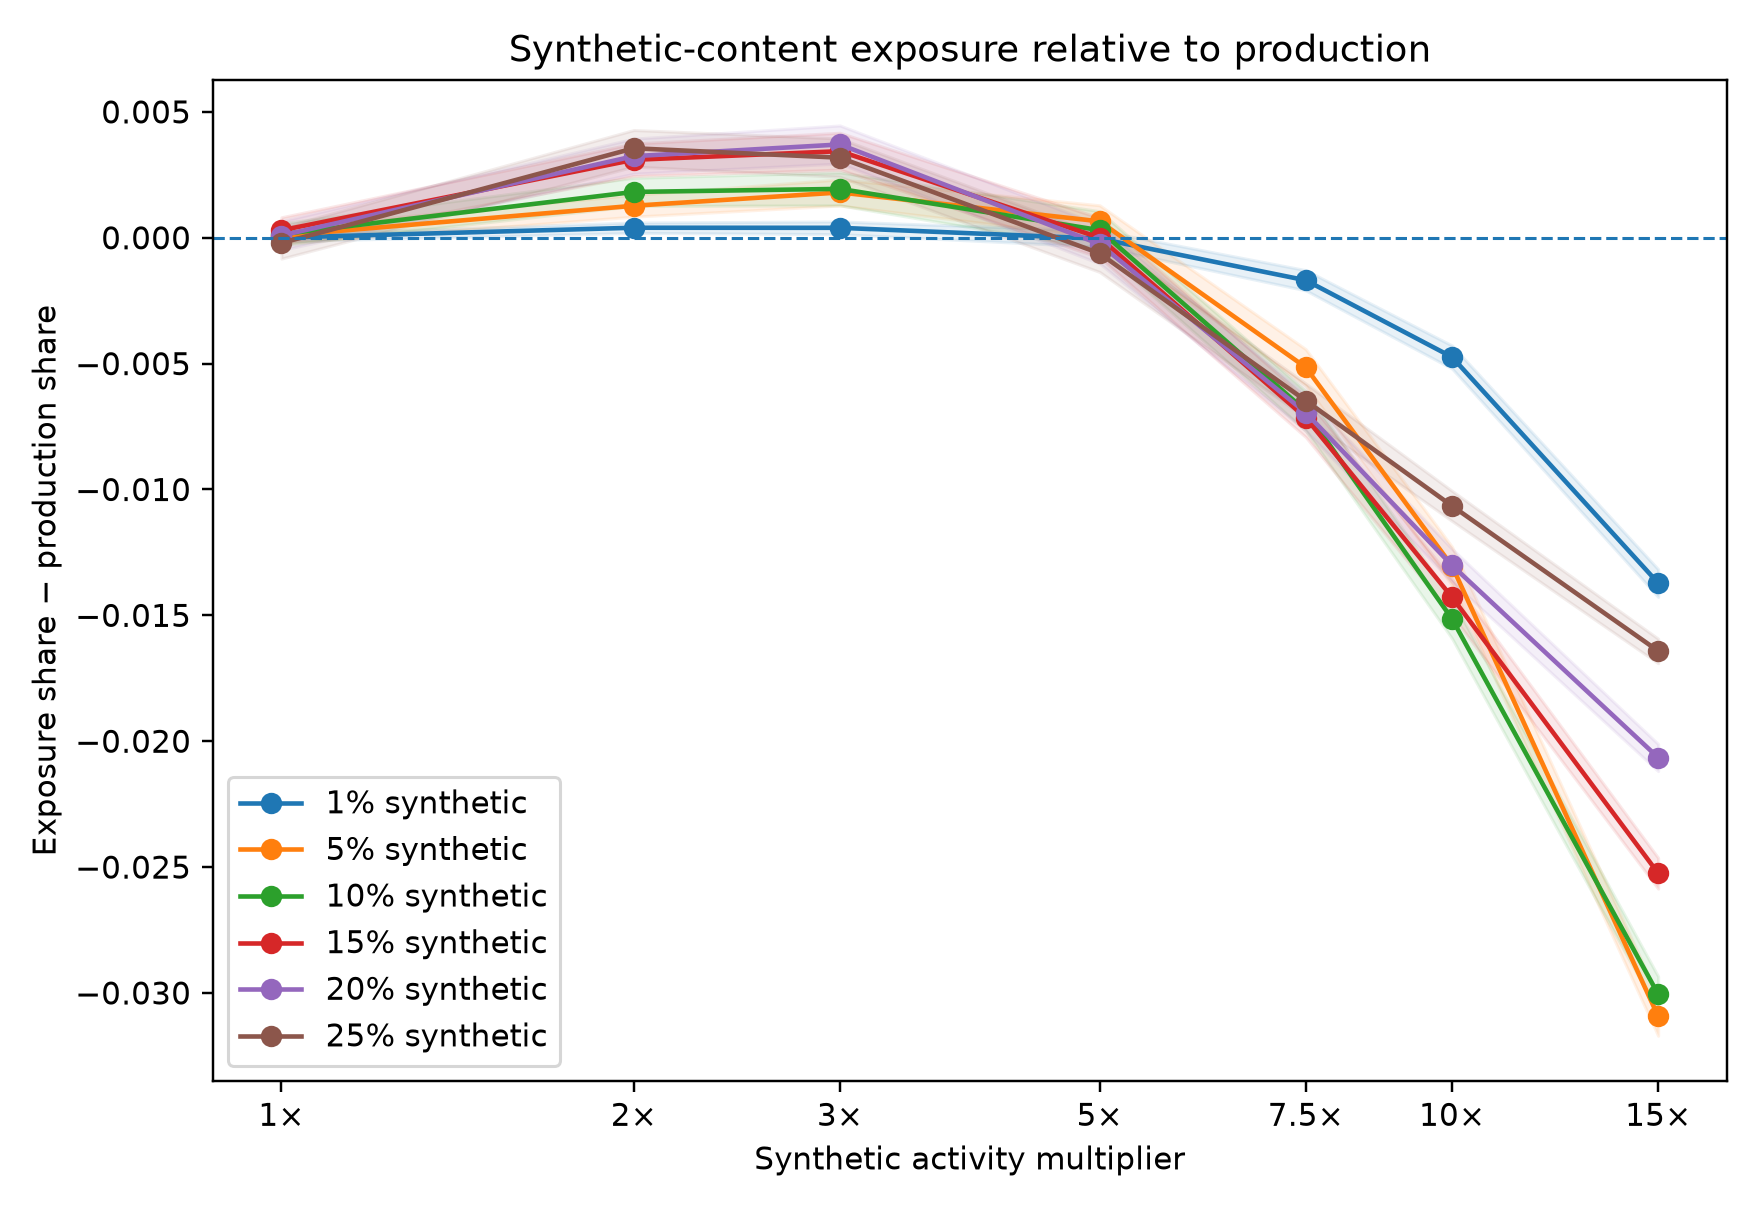
\includegraphics[width=0.9\linewidth]{imgs/alpha/D_vs_activity.png}
    \caption{\textbf{Relative synthetic exposure as activity increases.} Mean \(D=S_{\mathrm{exposure}}-S_{\mathrm{production}}\) across 10,000 independent worlds for each synthetic-producer prevalence and activity multiplier. Positive values indicate disproportionate synthetic exposure and negative values indicate attenuation. Shaded regions show 95\% confidence intervals.}
    \label{fig:D_vs_activity}
\end{figure}

The same pattern is visible across the full parameter grid in Fig.~\ref{fig:D_heatmap}. The largest mean \(D\) occurs at either \(2\times\) or \(3\times\) activity depending on prevalence. At \(7.5\times\) activity and above, mean \(D\) is negative for all tested prevalence levels. The magnitude of the effect varies with prevalence, but the overall turnover from small positive relative exposure at moderate activity to attenuation at high activity is present throughout the tested range.

\begin{figure}
    \centering
    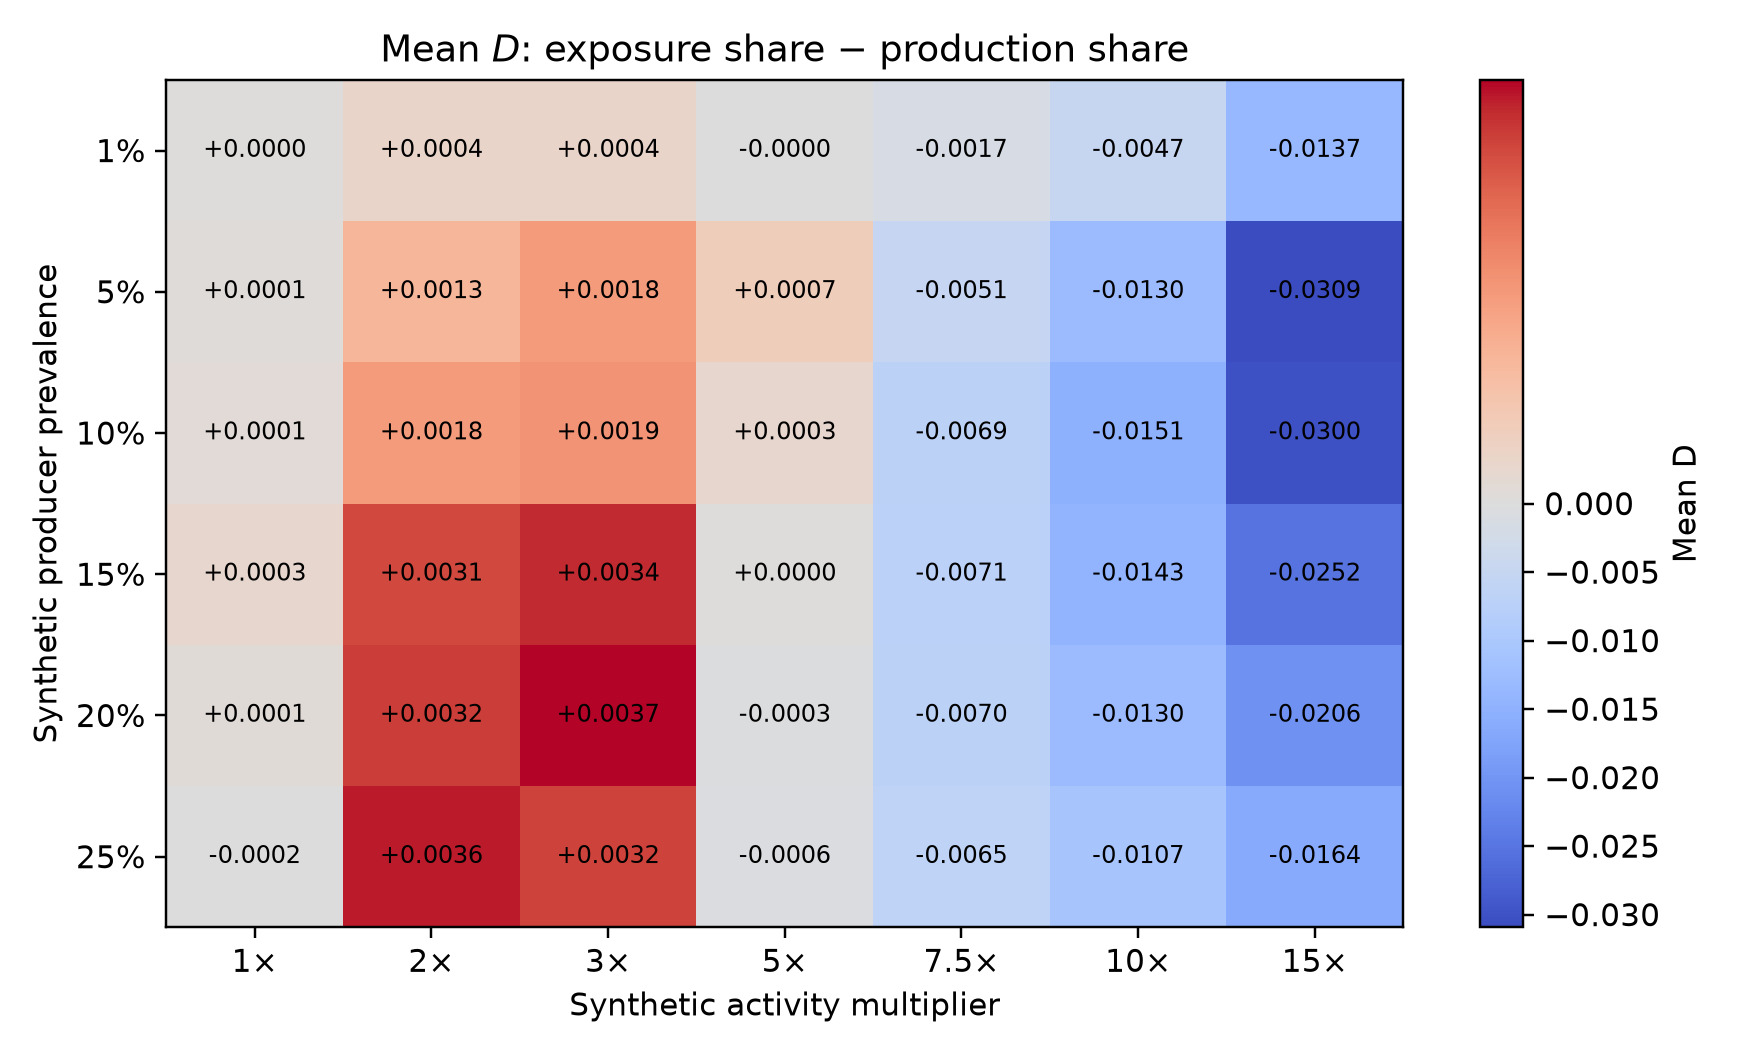
\includegraphics[width=0.9\linewidth]{imgs/alpha/D_heatmap.png}
    \caption{\textbf{Mean relative synthetic exposure across the experimental grid.} Each cell shows mean \(D=S_{\mathrm{exposure}}-S_{\mathrm{production}}\) across 10,000 independent worlds for the corresponding synthetic-producer prevalence and activity multiplier. Positive values indicate disproportionate exposure, while negative values indicate attenuation.}
    \label{fig:D_heatmap}
\end{figure}

The repeated-measures omnibus tests confirm that the relative-exposure outcome varies with both experimental factors. There is an effect of synthetic-producer prevalence, \(\chi^2(5)=869.53\), an effect of activity, \(\chi^2(6)=29176.50\), and a prevalence--activity interaction, \(\chi^2(30)=4042.40\); all three tests have \(p<0.001\). The interaction indicates that prevalence modifies the magnitude of the activity effect, although the qualitative non-monotonic pattern remains similar across prevalence levels.

The location of the turnover is also consistent across prevalence levels. The tested activity level with the largest mean \(D\) is \(2\times\) or \(3\times\), and linear interpolation between adjacent tested conditions places the subsequent zero crossing between \(4.67\times\) and \(5.28\times\). These values are descriptive interpolations within the simulated parameter grid rather than estimates of a universal threshold.

\begin{table}[t]
    \centering
    \caption{Turnover in mean relative exposure by synthetic-producer prevalence. Zero crossings are linearly interpolated between adjacent tested activity levels.}
    \label{tab:turnover}
    \begin{tabular}{rccc}
    \hline
    Prevalence & Peak activity & Peak mean \(D\) & Zero crossing \\
    \hline
    1\%  & \(2\times\) & 0.0004 & \(4.84\times\) \\
    5\%  & \(3\times\) & 0.0018 & \(5.28\times\) \\
    10\% & \(3\times\) & 0.0019 & \(5.11\times\) \\
    15\% & \(3\times\) & 0.0034 & \(5.00\times\) \\
    20\% & \(3\times\) & 0.0037 & \(4.87\times\) \\
    25\% & \(2\times\) & 0.0036 & \(4.67\times\) \\
    \hline
    \end{tabular}
\end{table}

The paired within-world contrasts support the same decline beyond the moderate activity peak. Table~\ref{tab:paired_3x_15x} reports the change in \(D\) from \(3\times\) to \(15\times\) activity. Mean \(D\) decreases at every tested prevalence, with the largest decline occurring at 5\% and 10\% prevalence. All reported contrasts remain significant after Holm adjustment, while the effect sizes indicate that the high-activity decline is substantially larger than the small positive exposure excess observed around the peak.

\begin{table}[t]
    \centering
    \caption{Paired within-world change in relative exposure from
    \(3\times\) to \(15\times\) synthetic activity. Negative values indicate
    lower \(D\) at \(15\times\). All contrasts have Holm-adjusted
    \(p<0.001\).}
    \label{tab:paired_3x_15x}
    \begin{tabular}{rccc}
    \hline
    Prevalence & Mean \(\Delta D\) & 95\% CI & \(d_z\) \\
    \hline
    1\%  & -0.0141 & [-0.0147,\,-0.0135] & -0.481 \\
    5\%  & -0.0327 & [-0.0336,\,-0.0318] & -0.721 \\
    10\% & -0.0320 & [-0.0329,\,-0.0311] & -0.685 \\
    15\% & -0.0287 & [-0.0296,\,-0.0278] & -0.614 \\
    20\% & -0.0244 & [-0.0252,\,-0.0235] & -0.539 \\
    25\% & -0.0196 & [-0.0205,\,-0.0187] & -0.444 \\
    \hline
    \end{tabular}
\end{table}

Figure~\ref{fig:exposure_efficiency} shows how exposure efficiency changes with synthetic activity. At low to moderate activity, synthetic-origin posts receive a similar or slightly larger number of successful feed receipts per post than human-origin posts. At high activity, the exposure-efficiency gap becomes negative across the tested prevalence levels, indicating that the average synthetic-origin post receives fewer feed receipts than the average human-origin post. This pattern is consistent with diminishing exposure returns at high synthetic activity, although the present model does not isolate the precise mechanism producing the decline.

\begin{figure}[t]
    \centering
    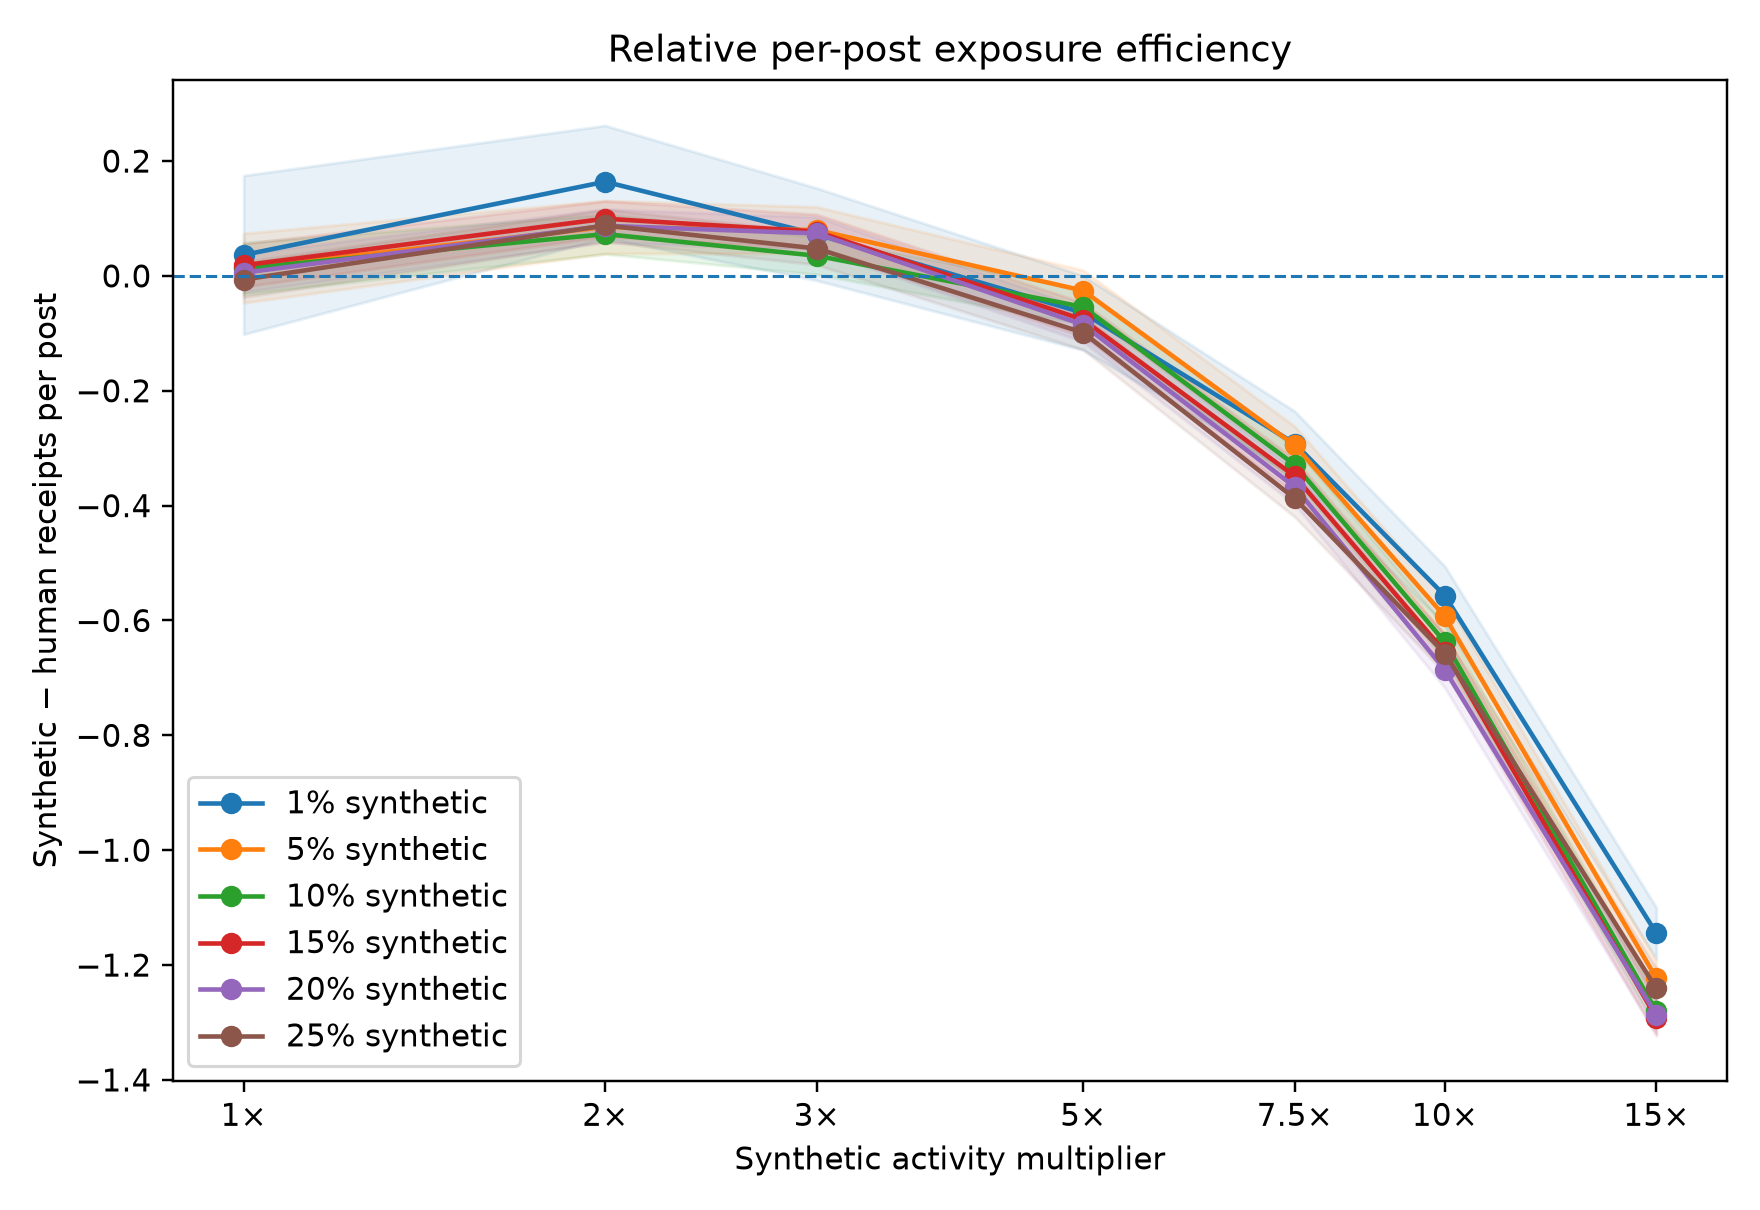
\includegraphics[width=0.9\linewidth]{imgs/alpha/exposure_efficiency_gap.png}
    \caption{\textbf{Exposure-efficiency gap across activity levels.}
    Difference in mean successful feed receipts per post between synthetic-origin
    and human-origin content. Positive values indicate higher per-post exposure
    efficiency for synthetic content, while negative values indicate lower
    exposure efficiency.}
    \label{fig:exposure_efficiency}
\end{figure}

Figure~\ref{fig:zero_receipt_gap} provides a second view of declining per-post exposure at high activity. At moderate activity, synthetic-origin posts are approximately as likely as, or slightly less likely than, human-origin posts to receive no feed receipts. At high activity, particularly at larger synthetic prevalence, synthetic-origin posts become increasingly more likely to receive zero feed receipts. This is consistent with greater competition for limited diffusion opportunities, but does not by itself identify the causal mechanism.
\begin{figure}
    \centering
    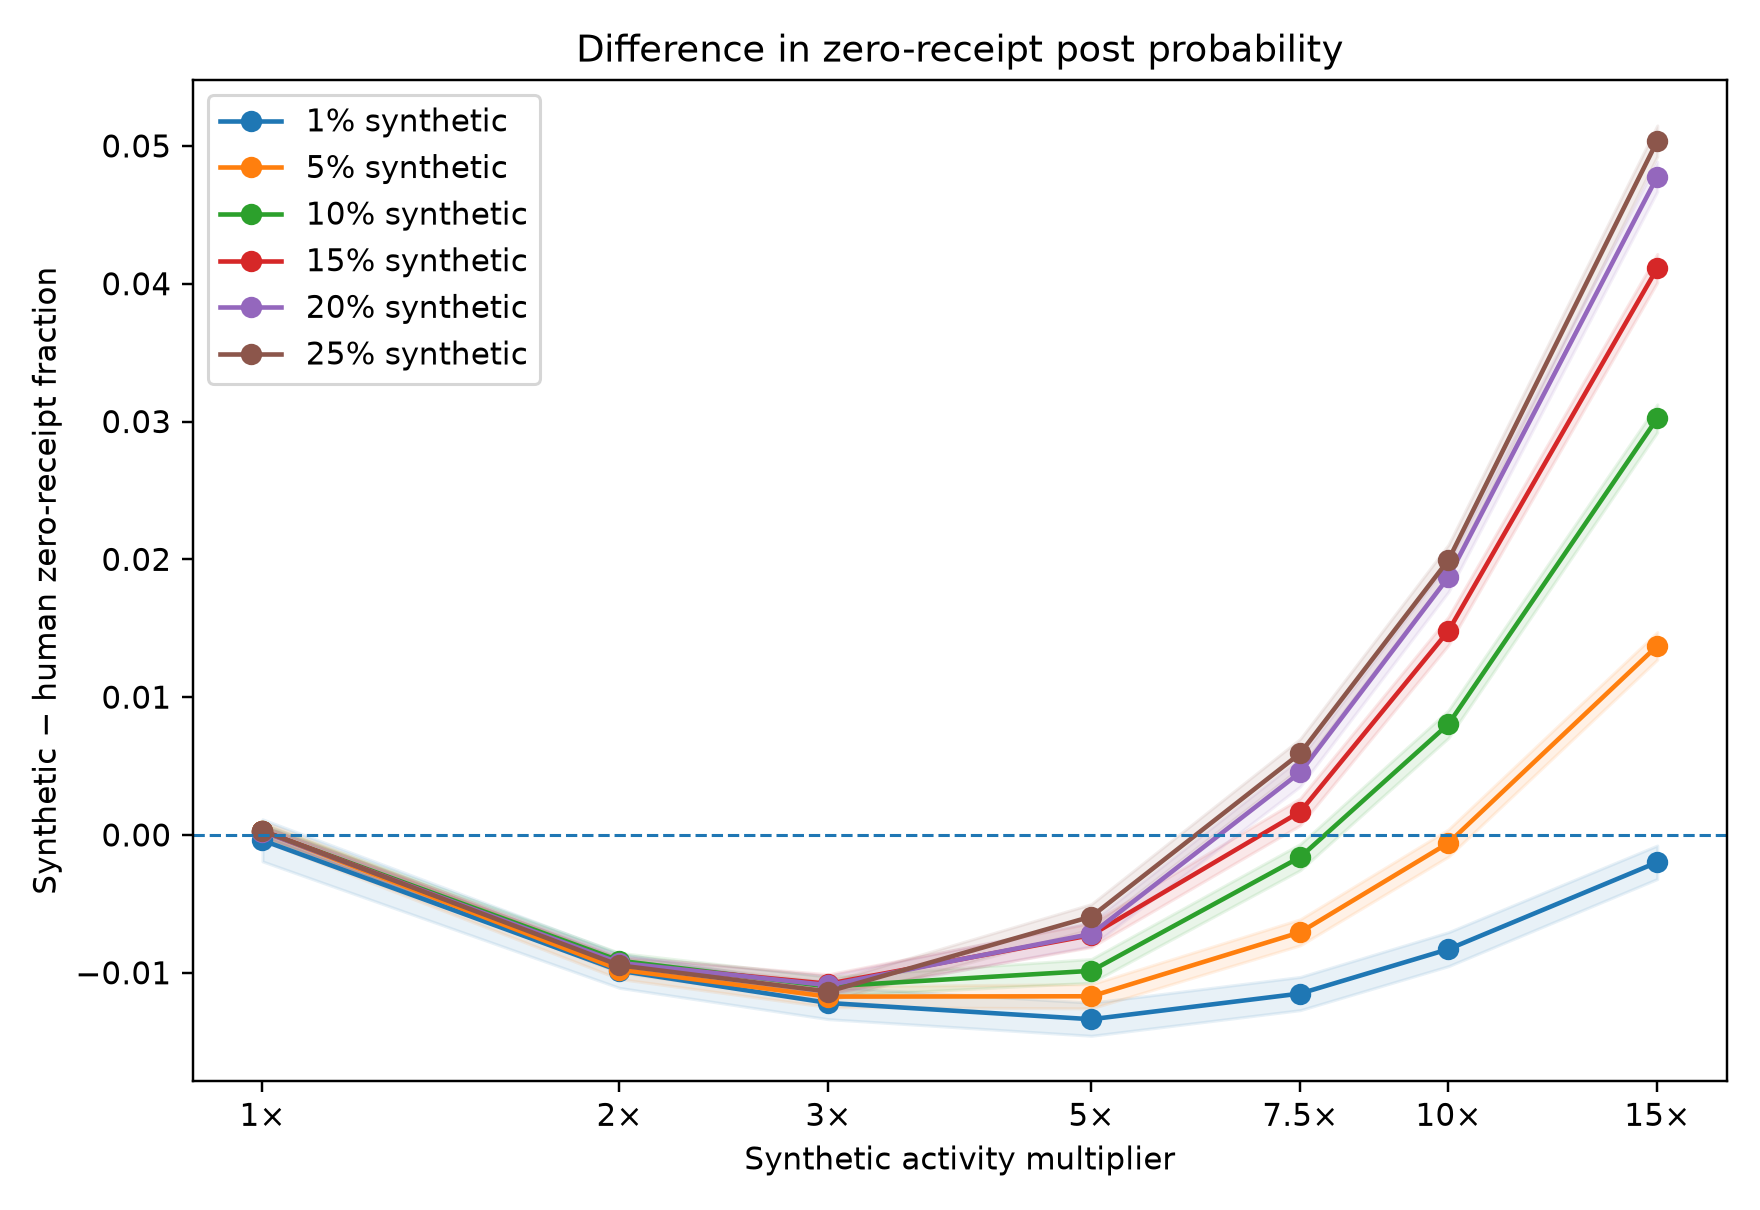
\includegraphics[width=0.9\linewidth]{imgs/alpha/zero_receipt_gap.png}
    \caption{\textbf{Difference in zero-receipt probability between synthetic and human posts.} Positive values indicate that synthetic-origin posts are more likely than human-origin posts to receive no successful feed receipts.}
    \label{fig:zero_receipt_gap}
\end{figure}

Figure~\ref{fig:convergence} shows that the estimates become increasingly stable as the number of independent worlds increases. The maximum absolute difference between checkpoint means and the final 10,000-world means generally decreases with sample size, while the maximum 95\% confidence-interval half-width narrows steadily. By 5,000 worlds, the maximum deviation from the final condition means is below \(0.001\). The 10,000-world point is omitted from the blue curve because its deviation from the 10,000-world reference mean is zero by construction. The convergence analysis therefore indicates that increasing the sweep to 10,000 worlds primarily reduces Monte Carlo uncertainty rather than changing the qualitative pattern of the results.

\begin{figure}
    \centering
    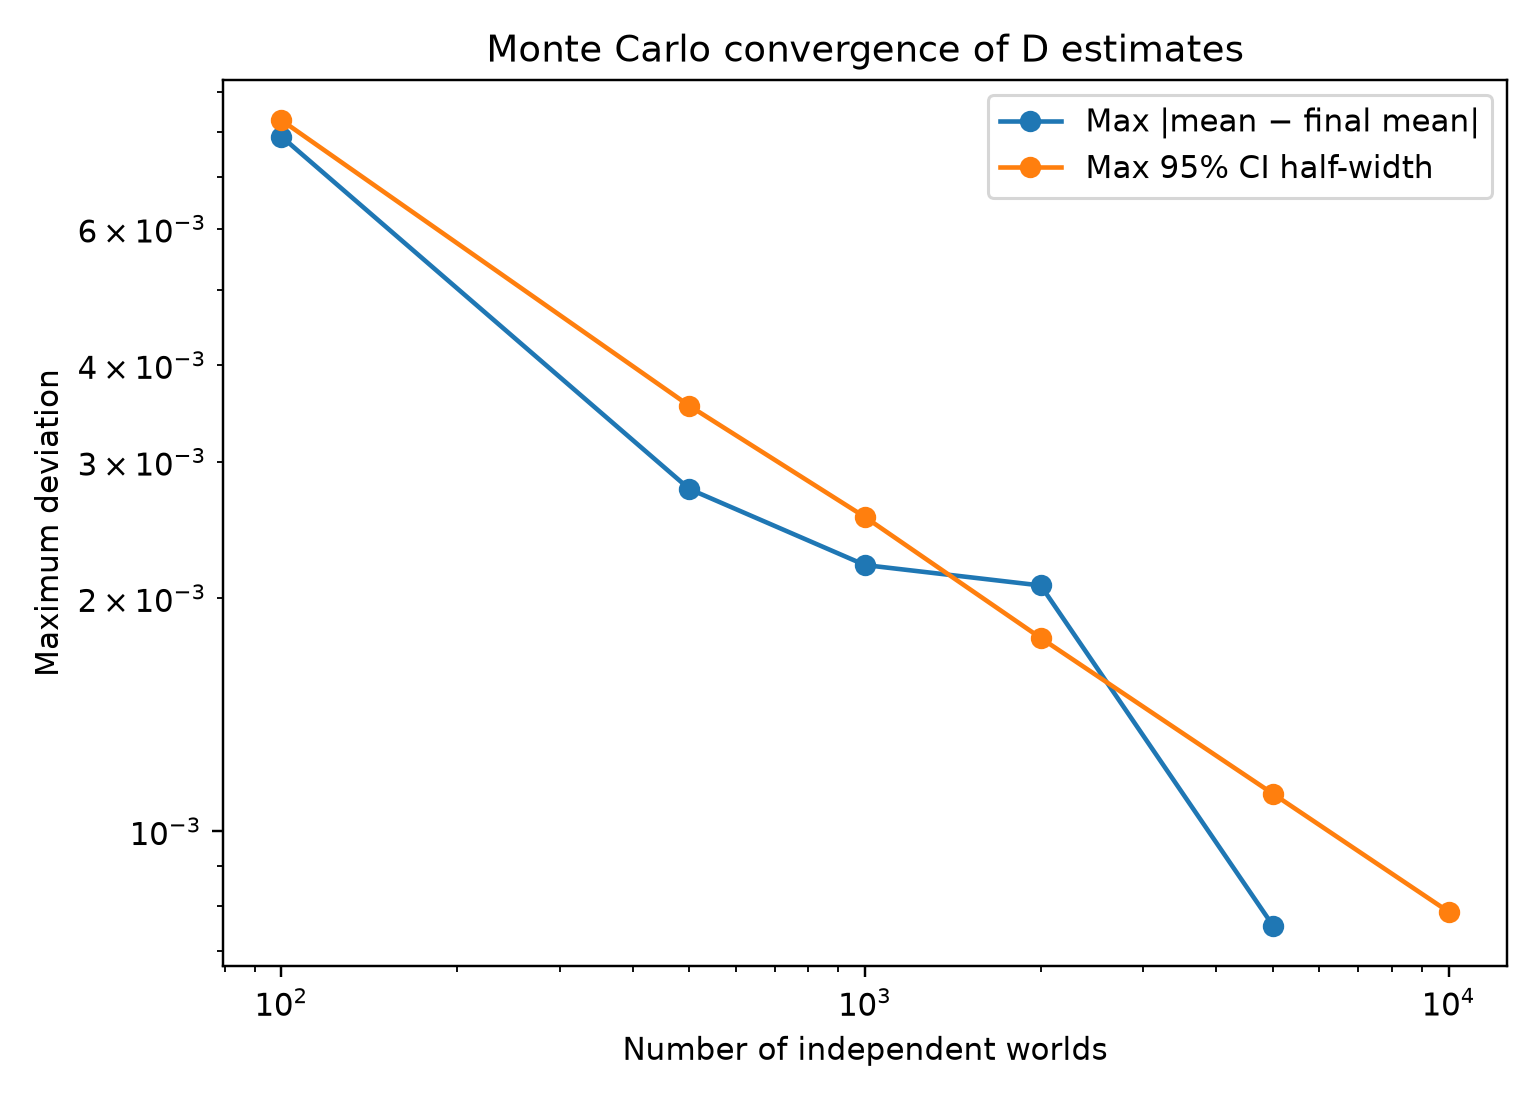
\includegraphics[width=0.9\linewidth]{imgs/alpha/convergence.png}
    \caption{\textbf{Monte Carlo convergence of D estimates.} The blue curve shows the maximum absolute deviation of condition means from the corresponding 10,000-world estimate; the 10,000-world point is omitted because its deviation is zero by construction. The orange curve shows the maximum 95\% confidence-interval half-width.}
    \label{fig:convergence}
\end{figure}

\FloatBarrier
\subsection{Feed-capacity sensitivity}
\label{sec:feed-results}

The focused experiment contains all 3,600 planned condition-runs, with 200 worlds in each condition. Figure~\ref{fig:feed-capacity} and Table~\ref{tab:feed-capacity} show substantial capacity dependence. At \(15\times\), mean \(D\) is negative in all six prevalence--capacity combinations. For example, at 5\% prevalence it is \(-0.0304\) with a one-item feed, \(-0.0050\) with a five-item feed, and \(-0.0508\) with a 20-item feed. Increasing capacity therefore does not simply weaken attenuation.

\begin{figure}[!htbp]
\centering
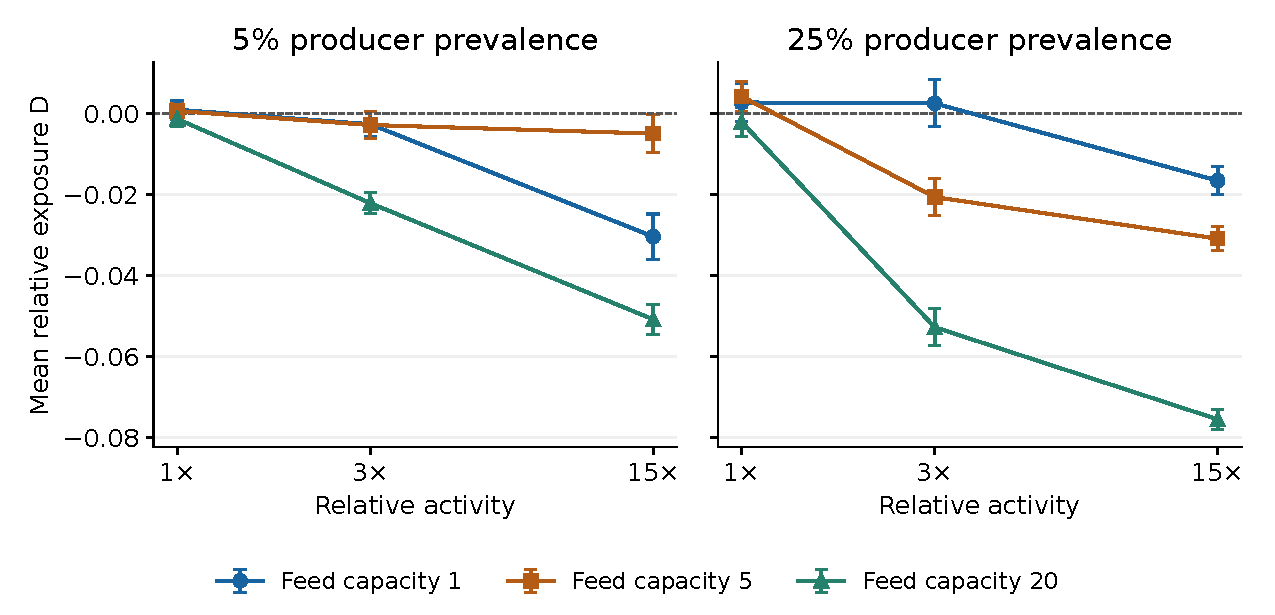
\includegraphics[width=\linewidth]{imgs/robustness/feed_capacity.pdf}
\caption{\textbf{Feed-capacity sensitivity.} Mean relative exposure and pointwise 95\% confidence intervals across 200 independent paired worlds. Lines connect the three tested activity levels for readability; they do not estimate intermediate values or a turnover threshold.}
\label{fig:feed-capacity}
\end{figure}

\begin{table}[!htbp]
\caption{Feed-capacity sensitivity across 200 paired worlds. Condition means and paired changes in $D$ use the same worlds. Intervals are pointwise 95\% $t$ intervals, without multiplicity adjustment.}
\label{tab:feed-capacity}
\centering\small
\begin{tabular}{rrrrrl}
\hline
Prevalence & $\alpha$ & Mean $D_3$ & Mean $D_{15}$ & Mean change & 95\% CI \\
\hline
5\% & 1 & -0.0027 & -0.0304 & -0.0277 & [-0.0336, -0.0218] \\
5\% & 5 & -0.0028 & -0.0050 & -0.0021 & [-0.0077, 0.0034] \\
5\% & 20 & -0.0221 & -0.0508 & -0.0287 & [-0.0330, -0.0244] \\
25\% & 1 & 0.0025 & -0.0166 & -0.0191 & [-0.0256, -0.0126] \\
25\% & 5 & -0.0206 & -0.0309 & -0.0103 & [-0.0154, -0.0052] \\
25\% & 20 & -0.0527 & -0.0755 & -0.0227 & [-0.0275, -0.0179] \\
\hline
\end{tabular}
\end{table}


All six mean paired contrasts \(D_{15}-D_3\) are negative. Five pointwise intervals exclude zero. For the five-item feed at 5\% prevalence, however, the mean change is \(-0.0021\), with interval \([-0.0077,0.0034]\); this comparison does not resolve a decline. At 25\% prevalence the same contrast is \(-0.0103\), with interval \([-0.0154,-0.0052]\). These exploratory intervals have no multiplicity adjustment.

The small positive effect at moderate activity in the main sweep is not consistently reproduced in the sensitivity sample. With a 20-item feed, mean \(D_3\) is already negative at both prevalences. The 200-world one-item-feed sample also does not resolve the small positive \(D_3\) seen in the 10,000-world sweep. The focused experiment therefore supports high-activity attenuation in the tested settings, but not a capacity-independent moderate-activity peak or zero crossing near \(5\times\).

\FloatBarrier
\section{Discussion}

For the main one-item-feed configuration, the results answer SQ1--SQ3 with a non-monotonic relationship between synthetic-agent activity and relative synthetic exposure. Moderate increases in activity produce a small positive value of \(D=S_{\mathrm{exposure}}-S_{\mathrm{production}}\), but this effect reverses as activity increases further. Across all tested synthetic-producer prevalence levels, mean \(D\) becomes negative at high activity. The exposure share grows less than production share at high activity in this configuration. Negative \(D\) does not mean that absolute synthetic exposure or its share has fallen.

This distinction between production and exposure is central to the result. Synthetic producers can account for a large amount of content simply because they act more frequently, even when their content receives less exposure per post than human-origin content. A high synthetic share of feed receipts should therefore not automatically be interpreted as evidence that the diffusion process disproportionately amplifies synthetic content. Production volume, overall exposure, and exposure relative to production are separate quantities.

For SQ2, producer prevalence changes the magnitude of this relationship while the main-sweep means retain the same broad shape. The omnibus analysis shows effects of prevalence, activity, and their interaction, while the turnover remains visible from 1\% through 25\% prevalence. For SQ3, the tested peak occurs at either \(2\times\) or \(3\times\) activity, and the interpolated zero crossing remains close to \(5\times\) across the tested prevalence range. These similarities suggest that the reversal is not restricted to one particular synthetic population size. The interpolated values should nevertheless be interpreted only within the present model configuration and not as real-world activity thresholds.

The per-post exposure results show how the turnover manifests at the post level: at high synthetic activity, synthetic-origin posts receive fewer successful feed receipts per post. Because this exposure-efficiency measure is closely related to \(D\) by construction, it should not be interpreted as independent causal evidence. The zero-receipt analysis provides a complementary distributional observation: at high activity, synthetic-origin posts increasingly receive no feed receipts. Together, these patterns are consistent with increasing competition for limited diffusion opportunities as production rises. However, the current measurements do not separately observe failed receiving attempts, feed displacement, repost opportunities, or changes caused by rewiring. We therefore treat competition for limited attention as a plausible interpretation rather than an identified causal mechanism.

The feed-capacity test narrows this interpretation further. Attenuation at high activity is not confined to a one-item feed, but changing capacity does not produce a simple monotonic change in the effect. The positive moderate-activity excess and the descriptive zero crossing from the main sweep should not be generalized to larger feeds. Because capacity also changes background initialization, repost order, and suppression of repeat receipts, these results do not identify feed displacement as the cause.

The result also illustrates why a multi-agent model is useful for this question. The intervention itself is simple: synthetic agents are activated more frequently while all other behavioural rules remain unchanged. Despite this monotonic increase in individual activity, the network-level exposure effect changes direction. The reversal therefore emerges from interactions between posting, reposting, filtering, limited feeds, opinion dynamics, and adaptive network structure rather than being specified directly in the synthetic-agent behaviour.

The connection to Tang et al.~\cite{tang2026} and Pendergrass et al.~\cite{pendergrass2025} is a modelling motivation, not a test of their full accounts of AI-slop production. Within the model, additional production need not maintain the same exposure efficiency. The Oliveira et al.~\cite{oliveira2026} framework makes this distinction observable because content diffusion depends on repeated interactions with recommendation, reposting, feed capacity, and network adaptation.

\subsection{Limitations and future work}

Several assumptions limit external validity. We use a random follower network, fixed innovation and receiving rules, and a fixed finite event horizon. Producer labels do not encode content quality, generation cost, coordinated ownership, or feedback-driven strategy. The main sweep's 10,000-world precision reduces Monte Carlo uncertainty within this model; it does not validate the model against real platform data or establish a stationary long-run outcome. The feed-capacity sensitivity experiment covers only two prevalences and three activity levels, so it cannot establish a new activity threshold or full robustness across the original grid.

The link to AI slop is consequently partial. We implement activity heterogeneity, producer prevalence, persistent provenance, and the distinction between production and feed receipt. We do not implement the strategy--reward loop described in the motivating literature. Network adaptation changes who follows whom, while producer weights and content-generation rules remain fixed. A generic high-activity subgroup could produce the same results.

A next producer-level extension could let agents select among content formats or topics using recent per-post receipt rewards, with a fixed-strategy control. It would require an explicit reward definition, update rule, observation window, and separate validation. Increasing activation weights alone would not model format selection or learning. Alternative network structures, receiving filters, innovation rates, longer horizons, and background initialization controls should also be tested. These extensions would assess whether the activity effect remains informative when more of the AI-slop production process is represented.

\section{Conclusion}

We extended DOCES with weighted activity, post provenance, and receipt tracking to study a labelled producer subgroup. In the main sweep, 10,000 independent worlds and 42 positive-prevalence conditions show a non-monotonic relation between activity and relative exposure.

Moderate synthetic activity produces a small positive exposure excess, while high activity produces attenuation relative to synthetic production share. Across prevalence levels from 1\% to 25\%, the largest mean \(D\) occurs at \(2\times\) or \(3\times\) activity, with descriptive zero crossings near \(5\times\). At higher activity levels, synthetic-origin posts also receive fewer successful feed receipts per post.

In the focused 200-world sensitivity experiment, high-activity mean relative exposure is also negative at feed capacities 5 and 20. The moderate-activity pattern changes, and one of the paired activity contrasts remains unresolved. This extends the evidence for attenuation to the tested conditions without establishing a universal threshold.

The main implication is that synthetic production volume and relative exposure should not be treated as interchangeable. Large quantities of synthetic content can enter users' feeds through high production alone even when the average synthetic post receives diminishing exposure. The quantitative turnover is specific to the main configuration. The feed-capacity experiment directly tests one inherited assumption, while alternative networks, recommendation rules, and adaptive producer strategies require separate experiments. Our results concern activity and provenance; they do not establish how real AI-slop producers respond to engagement rewards.

\bibliographystyle{splncs04}
\bibliography{bibliography}
%
\end{document}
